% Optional owned figure; not input by the current V166 review.
% Use at the full6.5in text width; do not shrink below5.85in.
\begin{figure}[p]
\centering
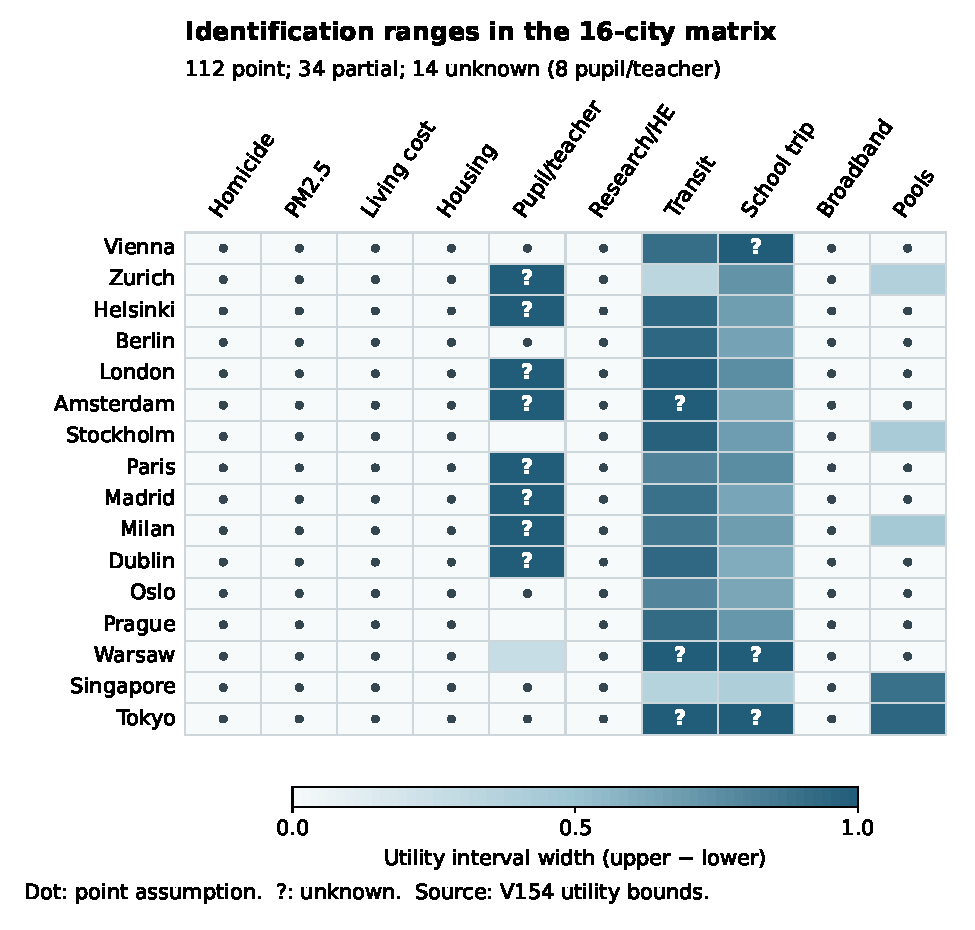
\includegraphics[width=\linewidth]{task4_v167_evidence_assets/identification_matrix.pdf}
\caption{Identification ranges in the retained sixteen-city, ten-indicator matrix.
Eight of the fourteen fully unknown entries concern upper-secondary pupil--teacher
ratios. Shading shows utility upper minus lower bounds; dots mark retained point
assumptions and question marks identify $[0,1]$ entries. Point assumptions include
submitted values and do not certify independent validation or zero measurement
error. These are identification bounds under the retained source rules, not
confidence intervals. Cities follow the input order. Source: V154 utility bounds.}
\label{fig:identification-matrix}
\end{figure}
